%! Author = charon
%! Date = 8/8/24

\subsection{Grundlagen des Mosquitto MQTT-Brokers}\label{subsec:mosquitto-mqtt}
Mosquitto ist ein Open-Source-Message-Broker, der das \gls{mqtt}-Protokoll implementiert.
\gls{mqtt} ist ein Publish/Subscribe-Protokoll, das für Netzwerke mit geringer Bandbreite,
hoher Latenz oder unzuverlässigen Verbindungen entwickelt wurde.
Es wird häufig in der \gls{iot}-Kommunikation verwendet, um Daten zwischen Geräten, Sensoren und Anwendungen auszutauschen.
\gls{mqtt}, und damit auch Mosquitto, baut auf dem \gls{tcp}/\gls{ip}-Stack auf, was eine zuverlässige Datenübertragung zwischen Client und
Server gewährleistet.
\gls{tcp} sorgt dabei für eine gesicherte, verbindungsorientierte Kommunikation, bei der Datenpakete in der richtigen
Reihenfolge und fehlerfrei übertragen werden.
Diese Basis auf dem \gls{tcp}/\gls{ip}-Stack macht \gls{mqtt} zu einem robusten und weit verbreiteten Protokoll für den Einsatz
in vernetzten Umgebungen, insbesondere im \gls{iot}-Bereich.
Mosquitto bietet eine Möglichkeit, \gls{mqtt}-Nachrichten zwischen verschiedenen Clients zu vermitteln.
Der \gls{mqtt}-Broker ermöglicht es Clients, Nachrichten an bestimmte Themen (Topics) zu senden (Publish) und/oder zu
empfangen (Subscribe).
Durch seine geringe Overhead-Belastung und die Unterstützung für \gls{qos}-Ebenen, stellt Mosquitto eine zuverlässige
Lösung für die Kommunikation in verteilten Systemen dar.
Es bietet auch erweiterte Funktionen wie Authentifizierung, Verschlüsselung (\gls{tls}) und Integration mit anderen
Diensten.\newline
Das Protokoll \gls{mqtt} definiert drei Arten von Nachrichten~\cite{mqtt}:
\begin{itemize}
    \item \textbf{Publish:} Ein Client sendet eine Nachricht an einen Broker, die dieser an alle Abonnenten weiterleitet.
    \item \textbf{Subscribe:} Ein Client abonniert ein bestimmtes Thema (Topic), um Nachrichten zu empfangen, die von anderen
          Clients zu diesem Thema gesendet werden.
    \item \textbf{Unsubscribe:} Ein Client beendet das Abonnement eines Themas und empfängt keine weiteren Nachrichten zu
          diesem Thema.
\end{itemize}
Der erste Schritt in diesem Zustand ist das Starten des \gls{mqtt}-Brokers.
Der Broker dient als Vermittler für die Nachrichten, die zwischen verschiedenen \gls{mqtt}-Clients ausgetauscht werden.
Dieser Schritt ist entscheidend für den weiteren Betrieb des Systems.
Nach dem Starten des \gls{mqtt}-Brokers geht das System in den Initialisierungszustand über.
Hier wird die Netzwerkschnittstelle initialisiert, die für die Kommunikation über \gls{mqtt} erforderlich ist.
Diese Initialisierung stellt sicher, dass das System in der Lage ist, sich mit anderen Geräten im Netzwerk zu verbinden
und Nachrichten zu senden oder zu empfangen.
Nach erfolgreicher Initialisierung wechselt das System in den Zustand \textit{Listening}.
In diesem Zustand wartet das System entweder darauf, dass es eine \gls{mqtt}-Nachricht empfängt oder es ist in einem Leerlaufzustand (Idle).
Dieser Zustand ist zentral für das System, da hier die Hauptoperationen entweder initiiert oder beendet werden.
Wenn eine MQTT-Nachricht empfangen wird, wechselt das System in den Verarbeitungszustand.
In diesem Zustand werden die empfangenen Nachrichten verarbeitet, und es kann entweder eine Nachricht veröffentlicht oder
das System kann sich für ein neues Thema (Topic) abonnieren~\cite{mqtt-manpage}.
Sollte die Verarbeitung eine Veröffentlichung erfordern, geht das System in den Zustand \textit{Publishing} über.
In diesem Zustand wird die verarbeitete Nachricht an den entsprechenden \gls{mqtt}-Topic veröffentlicht, sodass andere
abonnierte Clients diese empfangen können.
Alternativ kann das System in den Zustand \textit{Subscribing} wechseln, wenn die Verarbeitung das Abonnieren eines neuen Topics erfordert.
Dieser Zustand ermöglicht es dem System, Nachrichten von einem neuen Thema zu empfangen.
Wenn keine Nachricht zur Verarbeitung vorliegt, bleibt das System im Leerlauf.
Dieser Zustand wird auch erreicht, wenn alle anstehenden Aufgaben erledigt sind und das System auf neue Nachrichten oder Befehle wartet.
Sobald ein Herunterfahren (Shutdown) angefordert wird, wechselt das System in den Zustand Terminating.
In diesem Zustand werden alle notwendigen Ressourcen aufgeräumt, um das System ordnungsgemäß zu beenden.
Der endgültige Zustand des Systems ist \textit{Stopped}.
Nachdem alle Ressourcen bereinigt wurden, ist das System inaktiv und bereit, vollständig heruntergefahren zu werden.\newline
Diese Nachrichten werden über das \gls{tcp}-Protokoll zwischen Client und Broker ausgetauscht.
Der Broker verfügt über eine interne Datenstruktur, die die Themen und die zugehörigen Abonnenten speichert.
Diese Speicherung und das Weiterreichen dieser N
achrichten kann in einer State Machine abgebildet werden.
\begin{figure}[H]
    \centering
    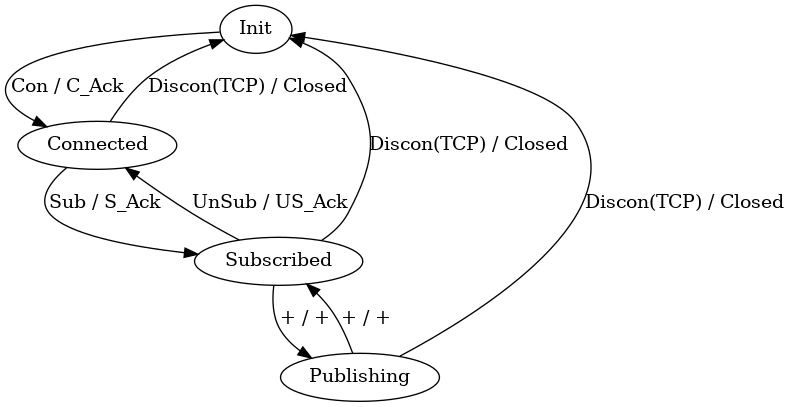
\includegraphics[width=\textwidth]{img/state_machine}
    \caption[State Machine des MQTT-Protokolls]{State Machine des Mosquitto MQTT-Protokolls. Sie beschreibt alle Zustände, die der Broker nach Empfangen von
    Nachrichten durchläuft. Beginnend mit der Überprüfung der Nachricht, über das Weiterleiten der Nachricht an die Abonnenten,
    bis hin zum Senden der Nachricht an die Clients.}
    \label{fig:mqtt_state_machine}
\end{figure}
\noindent Die Abbildung~\ref{fig:mqtt_state_machine} zeigt eine Zustandsmaschine (State Machine) für das \gls{mqtt}-Protokoll und beschreibt den Übergang zwischen
verschiedenen Verbindungszuständen eines \gls{mqtt}-Clients.
Diese Zustandsmaschine veranschaulicht, wie der \gls{mqtt}-Client in verschiedenen Situationen reagiert, z.B.\ beim Verbinden,
Abonnieren, Veröffentlichen und Trennen der Verbindung.\newline
Der Ausgangszustand der \gls{mqtt}-Zustandsmaschine ist der Init-Zustand.
Hier befindet sich der \gls{mqtt}-Client, bevor eine Verbindung zum Broker hergestellt wird oder nach einer Trennung.
Es ist der Ausgangspunkt und auch der Zustand, zu dem der Client nach einer Trennung zurückkehrt.
Wenn der Client eine Verbindung zum Broker herstellt (Con), wird ein Verbindungsbestätigungsnachricht (C\_Ack) empfangen
und der Zustand wechselt zu Connected.
Bei einer Trennung der \gls{tcp}-Verbindung (Discon(\gls{tcp})) wechselt der Zustand zu Closed.
In diesem Zustand ist der Client erfolgreich mit dem \gls{mqtt}-Broker verbunden.\newline
Der Client kann jetzt Abonnement- und Veröffentlichungsaktionen durchführen.
Der Client sendet eine Abonnementanfrage (Sub) an den Broker und erhält eine Bestätigungsnachricht (S\_Ack).
Der Zustand wechselt dann zu Subscribed.
Bei einer Trennung der \gls{tcp}-Verbindung (Discon(\gls{tcp})) wechselt der Zustand zu Closed.
In diesem Zustand hat der Client erfolgreich ein oder mehrere Themen (Topics) abonniert.
Der Client ist nun in der Lage, Nachrichten von den abonnierten Themen zu empfangen.
Der Client kann eine Nachricht veröffentlichen.\newline
Nach jedem erfolgreichen Veröffentlichungsprozess bleibt der Client im Subscribed-Zustand oder wechselt für die Veröffentlichung
kurzzeitig in den Publishing-Zustand.
Der Client kann eine Abmeldung (UnSub) von einem Thema anfordern und erhält eine Abmeldebestätigungsnachricht (US\_Ack).
Der Zustand kehrt dann zu Connected zurück.
Bei einer Trennung der \gls{tcp}-Verbindung (Discon(\gls{tcp})) wechselt der Zustand zu Closed.
In diesem Zustand veröffentlicht der Client Nachrichten an die abonnierten Themen.\newline
Es ist ein temporärer Zustand, in dem die Veröffentlichung von Nachrichten erfolgt.
Nach der Veröffentlichung einer Nachricht kehrt der Client in den Subscribed-Zustand zurück, um weitere Nachrichten empfangen zu können.
Bei einer Trennung der \gls{tcp}-Verbindung (Discon(\gls{tcp})) wechselt der Zustand zu Closed.\newline
Dies ist ein Endzustand, der erreicht wird, wenn die Verbindung zwischen dem Client und dem Broker getrennt wird.
Der Client ist nun nicht mehr in der Lage, Nachrichten zu senden oder zu empfangen.
Wenn der Client die Verbindung zum Broker wiederherstellt, kehrt der Zustand zu Init zurück, von wo aus er den Verbindungsprozess
neu starten kann.
\begin{figure}[H]
    \centering
    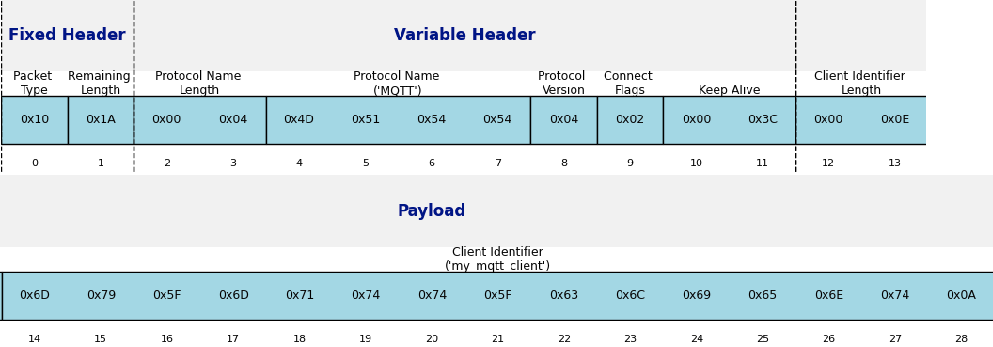
\includegraphics[width=\textwidth]{img/mqtt_packet_structure}
    \caption{Format einer \gls{mqtt}-Nachricht am beispiel eines Connect-Pakets.}
    \label{fig:mqtt_message_format}
\end{figure}
\noindent Die Struktur der zu sendenden Nachrichten ist von der verwendeten \gls{mqtt}-Version der Clients abhängig.
Die \gls{mqtt}-Version 3.1.1 -- die in dieser Arbeit verwendet wurde -- definiert ein festes Header-Format, das aus einem
Steuerbyte und einer variablen Länge besteht.
Als Nächstes folgt ein Variabler Header, der weitere Information über die Länge des Protokollnamens und den verwendeten
Protokollnamen, sowie die verwendete Protokollversion und ein Connect-Flag-Byte enthält.
das zehnte und elfte Byte enthalten die Keep-Alive-Zeit, die die maximale Zeit in Sekunden angibt, die der Client auf eine
Antwort des Brokers warten soll.
Die restlichen Bytes enthalten die Client-ID, die Länge des Benutzernamens und den Benutzernamen selbst, die
Länge des Passworts und das Passwort selbst.
Die \gls{mqtt}-Nachrichtenstruktur~\cite{mqtt} ist in Abbildung~\ref{fig:mqtt_message_format} dargestellt.
\newline
Die gesendeten Nachrichten haben im kürzesten Fall eine Länge von 2 Bytes, wobei das Steuerbyte für einen Verbindungsabbau
gesendet wird und somit nur aus dem Fixed-Header besteht.
Die Obergrenze der Größe eines validen Nachrichtenpakets beträgt 256 Megabytes~\cite{mqtt}.